\chapter{Design}

\section{Portable Document Format}
In the context of text redaction, it is essential to consider the relevant components that make up a PDF document and influence security for direct redaction in the document. We consider the PDF document type which contains text data for both the font and the layout of each character (glyph) on a page. 

\subsection{Structure}
A PDF document can be split into 4 distinct parts: 
    \begin{figure}[h]
    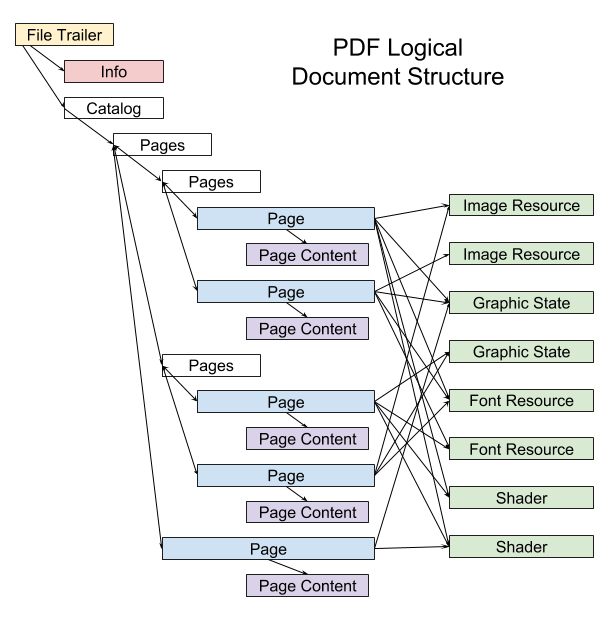
\includegraphics[width=0.6\textwidth]{latex/media/pdfstructure.png}
    \centering
    \caption{A overview of the structure of a PDF. It sort of represents a tree data structure with some irregularities. The actual content of the document is stored in the \textit{Page Content} where it is represented as a sequence of commands \href{https://skia.org/docs/dev/design/pdftheory/}{(image source)}.}
    \label{fig:tjexample}
\end{figure}\\
\textbf{Header}. The header of a PDF document serves as its starting point. It contains the critical information about the file which is essential for identifying the PDF format and ensuring compatibility with PDF readers. \\
\textbf{Trailer}. The trailer is found at the end of the document and provides essential information for reading and processing the document. It includes the number of entries in the cross-reference table. It references to the root object of the document's catalog, which contains information about the document's structure, outlines and elements. Finally it may include additional information about encryption, digital signatures and metadata if present. \\
\textbf{Cross-Reference Table(Xref)}. The Cross-Reference Table maintains a record of the location and structure of all objects within the PDF. The Xref table enables efficient random access and editing of the document. It lists the objects, their byte offsets within the file and information about whether an object is in use of has been deleted. \\
\textbf{Body}. The body is where the actual content resides. It includes everything that is visible within the document. This includes text, images, graphical elements, forms and more. The content of a PDF is organized into objects. 
\\\\
The actual contents of a page are often embedded through a stream. A stream may be contained in an object and consists of a sequence of operators with operands which may refer to other objects or information elsewhere.
\begin{figure}[h]
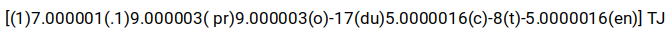
\includegraphics[width=0.85\textwidth]{latex/media/TJexample.png}
\centering
\caption{The TJ text showing operator specifies the glyphs to render, along with their widths and associated positional adjustments by the reference to a font object (not shown here). Adjustments are given in text space units. }
\label{fig:tjexample}
\end{figure}
\subsection{Text rendering}
PDF documents can render text in a wide range of ways, including by the use of a text showing operator such as TJ or Tj. The TJ operator takes as arguments a string of text and a vector of positional adjustments which displace the character with respect to its default position. This position is often determined by the previous character on the line, consisting of a fixed offset that is equivalent to the \textit{advance width} of the previous character. Figure \ref{fig:tjexample} is an example of a TJ text showing operator in practice.
\\\\
Glyph advance widths and glyph shifts create a security concern. The exact width of a redaction and any non-redacted glyph shifts conditioned on redacted glyphs may be used to eliminate potential redacted texts. \cite{bland2022story}. Documents may or may not have these positional adjustments based on the \textit{workflow} that has been used. When saving an email or using 'Save as PDF' in Microsoft Word for example, the documents have \textit{dependent} shifting schemes, while other workflows may produce documents which are \textit{unadjusted}.

\subsubsection{Redaction width}


\subsection{Metadata}
A PDF document may contain extra 'hidden' information which is contained within the metadata of the document. This metadata may contain information about the actual textual contents of the document (figure \ref{fig:metadataexmp}). An example are annotations by authors or reviewers which may comment on a specific part of the document, referring or quoting text which has been redacted from the page, but not from the document. 
\begin{figure}[h]
    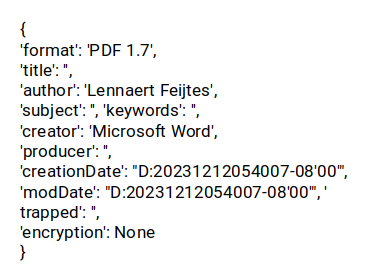
\includegraphics[width=0.5\linewidth]{latex/media/metadata.png}
    \centering
    \caption{An example of metadata which may be present in a PDF document. Information such as the author name, subject and description of the document can be retrieved if not also removed.}
    \label{fig:metadataexmp}
\end{figure}\\
The table of contents, embedded files, XML metadata and internal links are also hidden to the eye but may contain sensitive information even after redaction. This information may include author names, document descriptions, links or other references to sensitive personal information which has not been correctly removed.

\section{Steps of effective redaction}
\subsection{Labeling}
The process of safely redacting information from a document consists of multiple steps. To redact text, it first has be labeled as text that should be redacted in order to differentiate it from text that should not be removed. It is also important to differentiate between whole words and sub-strings of text elements so that exactly that what should be deleted is really removed from the document. Furthermore, a document can consist of multiple pages, so it should be known what set of possible redactions belongs to which page. 
\subsection{Locating}
The next step is locating the text that has to be removed. As mentioned, text is rendered by a sequence of commands in a content stream. The position of a text element and even an individual character can be reconstructed with these commands. In order to find the location of a text element the commands in the content streams have to be read, parsed and interpreted. There are various ways of rendering text in PDF documents, some more complex than others, and thus it requires a lot of research and work to handle all possible options. 
\subsection{Removal}
If text positions have been retrieved from a document, text can be removed. To redact, and thus to remove, text from a document, the commands that enable it to be rendered should be removed. Both the text rendering operation and other operations that may influence style and positioning should be removed completely. However, there is no guarantee that text is rendered in a certain way. Text on one line may consist of multiple text rendering operations or just one. Words may be individually grouped or each individual character is rendered separately. Again, this is dependent on the 'producer' of the file and the 'workflow' used. 
\\\\
\textbf{two images with examples of different text rendering styles based on found in the wild}
\subsection{Positional adjustments}
If text has been removed, possible positional information of characters of other words on the line have to be adjusted to reduce the leaked information. \textbf{More about this and how redaction is actually not saved after the document has been created} There are three ways to do this.
\subsubsection{Removing shifts}
Tools such as Edact-Ray protects vulnerable PDF redactions by providing a configurable level of information excisement to the user, allowing users to optionally remove all non-redacted glyph shifts. Spaces between words are rounded up to some width based on the width of a single character in the monospace font. These changes, while guaranteeing the redactions' security in general cases, change the document radically for the eye and may not be suitable in cases where style of the document has to be mostly preserved. 

\subsubsection{Multiple options}
It is possible to get the same general visual/aesthetic guarantees while making the adversary guess from a set of 10 names rather than one. If redacting a name, mixing in the shifts that would result from 10 other names at random from a given dictionary would increase the number of potential redacted, and would thus make it harder to guess the real redacted text. It would be necessary to devise to scheme based on either a prototyping method, i.e. by generating text in Microsoft Word and save them directly by editing the docx format, or reconstructing Miscorsoft Word schemes.  

\subsubsection{Computationally harder}
It is possible to get the same general visual layout while making it computationally harder to guess the redacted text by adding adjustments to every or most of the characters. As with the previous method, devising a scheme would be necessary. An example would be rounding each shift to a discrete interval.

\subsection{white space removal (optional)}
Positions of text on the same line and after the redacted text may be corrected. Due to the aforementioned complexity of text rendering, it may be difficult to determine the initial position and the new position of the text. If applicable, text on the same line, including replacements texts, have to be labeled as \textit{to-be-repositoned}. New positions are based on the difference between all the original texts and the replacement texts; one or more redactions. 

\subsection{Metadata}
The last step is the search of to-be-redacted text values in the (xml) metadata, embedded files and annotations. Non XML-Metadata can be accessed through the trailer and consists of key-value pairs which contain plain-text and which can be easily manipulated. Annotations often are included in the visible text of PDF documents and consist of the same sequence of operations as other text. This is the case for Microsoft Word. Text should be removed from these annotations the same way as normal text. Finally, embedded files may be removed. 
